
\documentclass[12pt]{article}
\usepackage[margin=.9in]{geometry}
\usepackage{amsfonts}
\usepackage{amsmath,amsthm,amssymb}
\usepackage{graphicx,caption,subcaption,subfig}
\usepackage{graphics}
\usepackage[mathscr]{euscript}
\raggedright
\parindent = 0 cm
\parskip = 8pt
\numberwithin{equation}{section}

\begin{document}
\title{Reddit or Not\\ Final Report \\ Reddit }
\author{Mathew Arndt, Nicolas Bertagnolli and Micheal Matheny}
\date{}
\maketitle
\pagenumbering{arabic}
\newpage
  
\section*{Introduction}
		We had a change in direction after we realized that working with the windmill data would  be more difficult than we had imagined.  The data was so large that we could not effectively manage it in memory. This meant that our project would focus on streaming algorithms or matrix sketching.  We decided that it might be more fun to actually look at aspects of the data instead of how to work with really really big data.  This project now uses reddit data which is collected in real-time from current posts.  \newline
		
		Reddit is a very rich site where users are allowed to post just about anything.  We were interested in looking at relationships between the users of reddit and their posts.  The hope was that we might be able to uncover interesting relationships that could lead to better modeling of internet forums.  Our analysis consisted of examining three different questions. The first question is, "How similar are high ranking posts?"  To asses this we examined the Jaccard Similarity of varying n-grams.  If we could uncover some degree of similarity between high ranking posts it might be possible to predict if a post is going to get a lot of likes. Next we asked, "Do users post in similar categories?"  To test this idea we clustered the data based on users to see if similar users post in the same subreddits.  This allowed us to look at relationships among users.  This could  potentially help answer questions like, "is user A similar to user B?"  It could also be used to create a low dimensional embedding of the users, similar to word vectors.  This might be helpful as a pretraining step in some larger learning system. Lastly we asked, "Are there words that appear frequently in specific subreddits." To test this we run Misra-Gris on the data and remove common words like "the," "and," "but," etc.  This will tell us if specific areas in reddit use common diction.  With this we might be able to identify the important words that categorize most of reddit's usage.
		
		
\subsection*{Parsing Reddit Data (Michael Matheny)}
Reddit is very unique in that it provides an easy interface for people to write bots and even actively encourages
the mining of their data. They do impose rate limits of 1 request per 2 seconds which can make data mining a bit slow
in some cases. The data of every reddit page can be viewed as a json file and there is an easy to use wrapper called Praw
that provides a high lever interface for building reddit bots. 
For this project we didn't need all the functionality that Praw offered, so we wrote a wrapper around some of Praw
allowing us to stream tuples containing only relevant comment data belonging to a particular subreddit. 

\begin{tabular}{|c|c|}
	\hline tuple info & Explanations \\
	\hline body &    The comment text \\ 
	\hline gilded &  Whether this comment was given gold \\ 
	\hline score &   The number of upvotes/downvotes \\ 
	\hline utc &     The time the comment was posted \\ 
	\hline subreddit &  The name of the subreddit \\ 
	\hline author &  The user of the comment writer\\ 
	\hline submission\_title &  The title of the submission that the commentator posted under  \\ 
	\hline submission\_author &  ... \\ 
	\hline submission\_score &  ...\\ 
	\hline submission\_utc &  ...\\ 
	\hline 
\end{tabular} 

We also wrote a lower level higher performance implementation for parsing user comments using the python requests 
library. 
		
		
\section*{N-Gram Analysis (Nicolas Bertagnolli)}
	To answer the question, "how similar are high ranking posts?" we take a set of 1000 reddit posts that have over 100 up-votes from all of reddit.  The threshold was determined using domain knowledge of reddit with the intent to adequately capture reasonably "good" posts.   We validated this threshold by calculating the average number of up-votes on a random sample of reddit posts (97 up-votes on average).  This says that when we take posts that score above 100 we are taking posts that are more or less well liked.   The (1-4)-grams for these 1000 posts were found and the pairwise Jaccard similarity was calculated.  The similarity was averaged and examined.  We found that the average Jaccard similarity between high ranking reddit posts for different n-grams when tested on all of Reddit was:\newline
	\begin{table}[h!]
	  \begin{tabular}{c | c c c c}
	  n-gram & 1 & 2 & 3 & 4\\
	  \hline
	  Similarity & .025 & $2.24e^{-3}$ & $1.75e^{-3}$ & $1.57e^{-3}$
	  \end{tabular}
	\end{table}
	
	These numbers are very low but they make sense because there is a great deal of variability in high ranking posts on reddit.  Take these two for example:\newline
	
	"Politics and opinions of the law aside, when a citizen has a complaint, they are encouraged to contact their representatives.  This sort of dickhead response deserves public shaming. Of course, he'll surely claim his email was hacked."\newline
	
	and \newline
	
	"If only he had another one"
	
	The first is fairly long , and the second is only a few words.  This in and of itself ensures low similarity just based on size.  Not to mention, that they both don't share a single word.  As it stands now we can say that the words alone do not make good predictors of reddit likeability.  However, there was a lot of variance in the rankings of these 1000 posts. We refined our question by restricting the posts to a range and asking, "How similar are high ranking posts where the rankings differ by no more than 100 votes?" To test this we then examined what happened when reddit posts that received between 100 and 200 up-votes were analyzed.  We found that the similarities were:\newline
	
\begin{table}[h!]
	  \begin{tabular}{c | c c c c}
	  n-gram & 1 & 2 & 3 & 4\\
	  \hline
	  Similarity & .023 & $2.21e^{-3}$ & $1.69e^{-3}$ & $1.54e^{-3}$
	  \end{tabular}
	\end{table}
	This was surprising because it was slightly worse than the whole set.  This led us to believe that a measurable amount of the similarity came from the upper upper echelon of reddit posts.  To test this hypothesis we refined our search to posts which received more than 1000 votes.  We find that there is significantly more similarity among posts above 1000 up-votes.  These results are:\newline
	
	\begin{table}[h!]
	  \begin{tabular}{c | c c c c}
	  n-gram & 1 & 2 & 3 & 4\\
	  \hline
	  Similarity & .042 & .017 & .017 & .016
	  \end{tabular}
	\end{table}
	
	In these experiments all possible subreddits were sampled.  This gave us an idea of similarity across all of reddit, but it seems like there is a lot of variability among posts.  With all of the variety in reddit we wondered if restricting our space to a particular category would yield higher similarity.  For example, the posts in the funny category are probably more similar to each other than a mixture of posts from funny and say the science reddit.  We find that for the subreddits funny and science the similarities are:
	
		\begin{table}[h!]
	  \begin{tabular}{c | c c c c}
	  n-gram & 1 & 2 & 3 & 4\\
	  \hline
	  Funny & .038 & .017 & .015 & .014\\
	  Science & .494 & .397 & .394 & .394\\
	  worldnews & .054 & .022 & .021 & .020
	  \end{tabular}
	\end{table}
	However the Science category only had 5 results that were greater than 100
	
These results are pretty good.  They are almost on par with the above 1000 upvotes for all of reddit.   We attempted to repeat this experiment on all of the categories for posts above 1000 likes but in most of these categories we could not get the required 1000 posts.\newline

  To summarize we find that the words alone in posts do not give a good indicator of whether or not the post will be well liked.  We find that most of the similarity in posts comes from the upper echelons of liked posts.  We also found that there was higher similarity between posts in specific subreddits.  It would be interesting to explore these ideas further.  For example what is it about the much more liked posts that causes similarity?  Could there be some aspect of the post size?  Are they all coming from a specifica category?  Are they all dealing with a specific topic?  It might also be interesting to look at different ways of assessing similarity.  Could we use other methods like clustering to see if there are deeper relationships in these posts?

\subsection*{Clustering Users (Michael Matheny)}
We want to find groups of users with similiar interests. To do this we decided to sample reddit users and then cluster the users based on the number of comments that they had posted in each subreddit. 
\begin{figure}[h!]
	\includegraphics[scale=.4]{fish_94.png}
\end{figure}

\subsubsection*{Mining Users}
 We wrote a small script that requests random subreddits and then scrapes the first few pages. After approximately 5 hours we had around 250k usernames. Praw can be used to scrape user histories, but it takes about a minute per 25 user comments. 
 Writing our own parser using the requests python library sped this up to around 25 comments every 2 seconds. Each user can take up to 16 seconds, so we let the script run continuously on a EC2 VM and at the time of writing this we had 
 around 33k user comment histories. 
\subsubsection*{Clustering Users}
To cluster the user data we represent each user as a vector where the number of comments in a subreddit gives 
the value at an index in the vector. The matrix containing all the user comments after removing 
deleted users is approximately 20000 users by 30000 subreddits, but it is extremely sparse with only around .1 \%
of the elements nonzero. 
We use cosine distance as our distance metric for the data since we only want to compare users interests. 

We initially clustered the data using the scikit learn cluster library, and experimented with numerous different 
methods and distance functions. We found that for this data cosine similarity seems to provide the most interesting 
and relevant clusters which makes sense since we only care about user interests and not the number of comments 
they produced.

As the data got larger many of clustering method began failing, taking too long, or 
would run out of memory. The only methods in scikit that work for this are Kmeans, Kmeans batch, and DBSCAN. 
DBSCAN clusters by density which doesn't make much sense for this data. Kmeans takes extremely long (10 minutes). 
Kmeans batch is extremely quick, but the quality of the clustering at times was significantly worse than Kmeans. 
We wanted to see if we could do better so we looked into several methods.
\begin{enumerate}
\item JLT: Calculations would suggest that we need to accept quite high error per data point for there to be a sizable dimensionality reduction:
 $$k = .01^{-2} \log(20000) = 99034$$
 $$k = .1^{-2} \log(20000) = 990$$
\item SVD: Since the data is very sparse computing the first few rows of the SVD is probably not too bad. 
\item Kmeans with LSH. 
\end{enumerate} 
Our implementation of Kmeans with LSH works by projecting each point onto a set of random vectors. Each random 
vector provides a single bit. For each point we keep $b$ bits grouped into $r$ integers. 
At the begining of each iteration of Kmeans LSH we hash all centroids into $r$ hash tables and then 
generate a list of the centers that each point collides with. The center that the point collides
with the most determines the points cluster. 

\subsubsection*{Results}
To compare implementations we found hyperparameters for each method that gave almost exactly the same 
 average distances between points and their cluster centers as vanilla Kmeans. We used $k = 100$ for all results. 
\begin{figure}[h!]
	\centering
	\begin{tabular}{|c|c|c|}
		\hline Algorithm & Parameters & Time (sec)\\ 
		\hline Kmeans Vanilla & - & 287 \\ 
		\hline Kmeans SVD & k = 60 & 13 \\ 
		\hline Kmeans JLT & k = 100 & 28 \\ 
		\hline Kmeans LSH & b = 6, r=30 & 283\\ 
		\hline 
	\end{tabular} 
\end{figure}
SVD and Kmeans are both written in C with python handles which makes comparing times between these algorithms a bit 
error prone. For instance the label assignment code that maps 
points to centers in LSH takes cumulatively around 210 seconds to run and most of this time is from a single max 
operation over a dictionary of counts. 
\subsubsection*{Clusters}
Below are some clusters we found as subreddit clouds where each word is a specific subreddit and the size is determined by its influence on the centroid.  It is interesting to note that these clusters are based solely on user posting habits.  We uncover relationships between users who like similar things.  One of the more "family friendly" examples is the fantasy sports cluster included below.  We find similar clusters for users who like professional sports, college sports, hockey, and many more. 
  
\begin{figure}[h!]
\centering
	
\includegraphics[scale=.2]{football_95.png}
\end{figure}

Most clusters we found for reddit users are small and around .2\% of
 the user base to maybe 1\%. Around a quarter of users only 
 post in the major default subreddits. Many of the remaining clusters 
 are focused on very specific interests such as My Little Pony, 
 aquariums, fantasy football, specific porn interests, or PC gaming. 
 It seems that many reddit users use their accounts for following a 
 specific interest or maybe have a throwaway account for things
 that they are not proud of. 
\begin{figure}[h!]
	\centering
	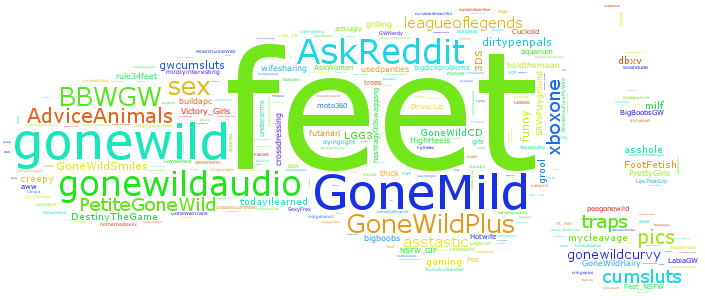
\includegraphics[scale=.4]{feet_16.png}
\end{figure}


	

\section*{Frequent Items Analysis (Mathew Arndt)}	
	
Here we ask the question, "Are there words that appear frequently in specific subreddits?"  To answer this question, the data mining seeks to find words that occur most frequent.  For each comment in the subreddit, the challenge was to collect, identify and record the most frequent words.  Since there were over one million possible words in the space and millions of comments per year for the domain space, this problem lends itself well to a streaming algorithm.  Streaming allows the algorithm to use as little storage space as possible which is critical for such a large element and domain space.  

Focusing on words that occur most frequently, \textbf{Heavy Hitter} algorithms were considered.  For our experiment, the \textbf{Misra-Gries} algorithm was then selected, mainly for its robustness and streaming model adaptation.  In fact, Python has a method named \textit{yield} which simply connects the parser to the Misra-Gries algorithm for recording.

To prepare our data we removed non-alphanumeric characters along with many common English words like "the," "if," "and," etc.   These were removed because they appear so frequently they detract from the actual meaning of our results.    As a remedy, a stop list was created with a list of words to be ignored.  This list was modified twice more.  First, the original list had to be duplicated because \textit{title case} continued to appear in the words.   We did not remove numbers and proper names from the posts because they often provide meaning, especially for certain subreddits.  Nevertheless, some experiments may consider removing these elements depending on the purpose of the mining.

Part of the experimental design was the selection of subreddits from which to mine.  With thousands of subreddits to select from, this is no trivial task.  Some of the more popular subreddits are \textit{funny, pics, videos, etc.}  The selection approach here was simple:  select subreddits that were popular yet had a concept that could be identified by its frequent words (topical bias hopefully excluded).   With that criteria in mind, experiments were run on the following subreddits: 

\begin{itemize} \itemsep1pt \parskip0pt \parsep0pt

  \item worldnews
  \item science
  \item funny
  \item movies
  \item aww
  \item gaming
  \item technology
  
\end{itemize}

Not all subreddits are as popular or as dense as the others.  Better results occur when the mining is allowed to traverse the comments in the subreddit to completion or near completion.  The algorithm was allowed to run until timeout.  

\begin{table}[h!]
\begin{tabular}{ll}
\textbf{subreddit} & \textbf{comments} \\
 \hline
funny              & 64,000           \\
worldnews          & 63,000           \\
gaming             & 51,000           \\
movies             & 39,000           \\
technology         & 22,000           \\
aww                & 16,000           \\
science            & 11,000          
\end{tabular}
\end{table}



For displaying the results, both tabular and histogram forms were considered.  In the end, a pictoral representation of the results was deemed best.  A \textit{wordle}, also known as a \textit{word cloud}, is such a representation where  greater prominence is given to words that appear more frequently.  Here is an example of one of the experiments run: 

\centering
The first \textbf{worldle} comes from the Misra-Gries output on the \textit{movies} subreddit:

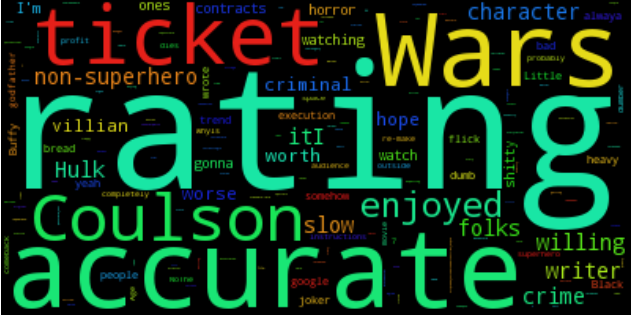
\includegraphics[scale=.5]{movies.png}

The second \textbf{worldle} comes from the Misra-Gries output on the \textit{movies} subreddit:
\centering
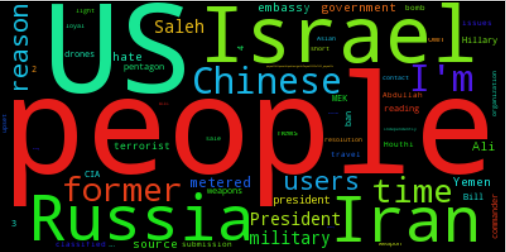
\includegraphics[scale=.5]{worldnews.png}

\raggedright

The \textbf{Misra-Gries} algorithm not only takes as input the stream of words but also the number of available counters, \textit{k}.  The number of counters has direct consequences on the accuracy of the Misra-Gries algorithm and also the number of words recorded and displayed.  The following shows the inverse relationship of the number of available counters and the error.    

\[k=\frac { 1 }{ \varepsilon  } \]  

or, in terms of error 

\[\varepsilon =\frac { 1 }{ k  } \]

For our experiments, a tradeoff exists between the accuracy in the algorithm and the amount of word clutter in the output.  In the end, the number of counters selected was two hundered, producing clean output and just a 0.5 percent error.

A basic rundown of the results of the experiments can be found below:

\begin{table}
\centering

\caption{Misra-Gries, k=200, \textit{movie} subreddit}
\begin{tabular}{c|c|c}
\hline
\textbf{word} & \textbf{frequency} & \textbf{proportion}\\
\hline
movie & 468 & 0.304\\
\hline
movies & 173 & 0.112\\
\hline
film & 113 & 0.073\\
\hline
I'm & 47 & 0.031\\
\hline
people & 27 & 0.018\\
\hline
superhero & 18 & 0.012\\
\hline
\end{tabular}
\end{table}

\begin{table}
\centering

\caption{Misra-Gries, k=200, \textit{worldnews} subreddit}
\begin{tabular}{c|c|c}
\hline
\textbf{word} & \textbf{frequency} & \textbf{proportion}\\
\hline
people & 284 & 0.095\\
\hline
US & 65 & 0.022\\
\hline
Israel & 24 & 0.008\\
\hline
Russia & 13 & 0.004\\
\hline
Iran & 12 & 0.004\\
\hline
Chinese & 12 & 0.004\\
\hline
\end{tabular}
\end{table}

Overall, the algorithm performed efficiently on the stream.  The main bottleneck was connecting to Reddit and the limitation on accessing the comments.  The stopwords did have an affect on which words were selected.  Short phrases might be more meaningful than single words because some context is lost in the concepts.  Also, the results were not as general as might be expected.  Proper names and places often showed up in the higher word frequency.  The \textit{k} = 200 worked well and produced clear wordles.  The main topic of the subreddit could possibly be determined by the most frequent words which is a good indicator of the effectiveness of the algorithm.   

  


\begin{figure}[h!]
	\centering
	
\includegraphics[scale=.6]{vegan_30.png}
\end{figure}




	
	
	

\end{document}